\newpage
\maketitle
\begin{center}
\Large \textbf{第5章 卡尔曼滤波} \quad 
\end{center}
\begin{abstract}
到目前为止,我们所讨论的基于协整模型的交易对策略,有一个重要的假设,即交易对之间的协整系数是不变的。但是在实际应用中,这些协整系数可能会发生缓慢的改变,如果我们用固定值,可能不会取得最佳的应用效果。在本章中,我们将采用State Space Model来解决这一问题,具体业讲,就是利用卡尔曼滤波技术,将交易对的对冲比例视为系统不可见的状态,将交易对中标的的收益率作为可观察项,利用卡尔曼滤波器的滤波功能,通过不断增加的新观测数据,利用贝叶斯推理,使我们能够更加精准的估计系统不可见状态,在本例中就是交易对的对冲比例。实际上,交易对的对冲比例,不仅会发生缓慢的变化,有时因为监管、宏观经济、市场事件等原因,交易对的对冲比例还可能发生剧烈的变化,这就需要我们识别市场所处状态,识别出市场状态的改变,从而做出更加科学的决策,这部分内容将在下一章隐马可夫模型章节中介绍。
\end{abstract}
\section{卡尔曼滤波}
\subsection{State Space Model概述}
在State Space Model中,我们要研究的对象是环境,这里就是市场。环境会处于某种状态,而且环境所处的状态随着时间而改变。但是我们不能直接观测到环境,我们只能得到一些观察,我们希望通过观察来推测出系统年处的状态。以我们当前的任务为例,我们的环境就是市场上的交易对,而状态就是交易对的对冲比例,而由于各种原因,如市场微观结构等,我们只能得到交易对标的的收益率,其中具有很大的噪声,信噪比很低,我们的任务就是通过观察这些收益率数据,得到交易对的对冲比例。
State Space Model可以用如下图形来表示:
\begin{figure}[H]
	\caption{通用State Space Model}
	\label{f000054}
	\centering
	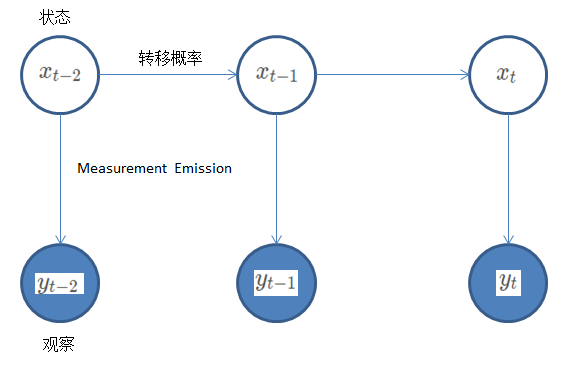
\includegraphics[height=10cm]{images/f000054}
\end{figure}
图中上面白色的圆圈代表环境的隐藏状态$x_{t}$,蓝色的圆圈代表环境的观测值$y_{t}$,系统会从一个状态转移到另一个状态,可以用一个概率$P(x_{t})x_{t-1}$来表示,环境所处状态决定观察值$P(y_{t} \vert x_{t})$,环境初始时的概率为$P(x_{0})$,根据这些变量的不同特性,我们可以把State Space Model分为四种类型:
\begin{table}[H]
\caption{State Space Model类型}
\label{t000001}
\begin{tabular}{|c|c|c|c|} \hline
名称 & $P(x_{t} \vert x_{t-1})$ & $P(y_{t} \vert x_{t})$ & $P(x_{0})$ \\ \hline  
离散模型(隐马可夫模型) & $A_{x_{t-1}, x_{t}}$ & Any & $\pi$ \\ \hline
线性高斯(卡尔曼滤波器) & $\mathcal{N}\big(  Ax_{t-1}+B, \theta \big)$ & $\mathcal{N}\big(  Hx_{t}+C, R \big)$ & $\mathcal{N}\big(  \mu _{0}, \epsilon _{0} \big)$ \\ \hline
非线性非高斯(粒子滤波器) & $f(x_{t})$ & $g(y_{t})$ & $f_{0}(x_{0})$\\ \hline
\end{tabular}
\end{table}
利用State Space Model可以做三件事情:
\begin{enumerate}
\item 预测:预测下一个到几个时刻的状态值;
\item 滤波:根据当前的观察值,预测系统状态;
\item 平滑:利用过去的观察值,解释过去状态变化情况;
\end{enumerate}
在这一章,我们所研究是线性高斯模型,即卡尔曼滤波器,我们同时会利用贝叶斯推断,通过不断增加的观察值,来逐步精确预测环境状态,在这里就是交易对的对冲比例。\newline
\subsection{数学原理}
在这一部分,我们将简单讲述卡尔曼滤波的数学原理,公式和符号会比较多,但是重点是理解其背后的数据直觉,不必纠结与具体推导过程。\newline
环境状态我们用一个向量来表示$\boldsymbol{x}_{t} \in R^{n}$,由于其会随时间变化,因此我们为其添加了下标$t$,因为卡尔曼滤波是线性高斯模型,当前时刻的状态,是由前一时刻的状态经线性组合再加上高斯噪声所组成,如下所示:
\begin{equation}
\boldsymbol{x}_{t} = A\boldsymbol{x}_{t-1} + \boldsymbol{b} + \boldsymbol{u}_{t}
\label{e000065}
\end{equation}
其中$A \in R{n \times n}$的矩阵,$\boldsymbol{b} \in R^{n}$,$\boldsymbol{w}_{t} \in R^{n}$为高斯白噪声。\newline
系统的观察用$\boldsymbol{y}_t \in R^{m}$表示,其由当前时刻环境状态的线性组合加高斯白噪声组成,如下所示:
\begin{equation}
\boldsymbol{y}_{t} = H\boldsymbol{x}_{t} + \boldsymbol{c} + \boldsymbol{v}_{r}
\label{e000066}
\end{equation}
系统初始状态为高斯分布:
\begin{equation}
\boldsymbol{x}_{0} \sim \mathcal{N} \big( \boldsymbol{\mu}_{0}, \Sigma _{0} \big)
\label{e000067}
\end{equation}
环境状态在t时刻噪声:
\begin{equation}
\boldsymbol{u}_{t} \sim \mathcal{N} \big( 0, \Sigma _{t}^{u} \big)
\label{e000068}
\end{equation}
环境观察在t时刻噪声:
\begin{equation}
\boldsymbol{v}_{t} \sim \mathcal{N} \big( 0, \Sigma _{t}^{v} \big)
\label{e000069}
\end{equation}
\subsection{PyKalman库介绍}
在这一节中,我们将讲述利用卡尔曼滤波来确定交易对的动态对冲比例。我们要研究的交易对为TLT和IEI,其面向美国债券市场,具有相同的市场因素,因此应该具有稳定的协整比例。在本节中我们将使用pykalman库,所以我们先来讲解一下在pykalman库中,卡尔曼滤波的表示方式,主要参考自\cite{r000003}。\newline
我们同样用$x_{t}$来代表环境的隐藏状态,用$y_{t}$来代表对环境的观察,则卡尔曼滤波可以表示为:
\begin{equation}
\boldsymbol{x}_{0} \sim \mathcal{N} \big( \boldsymbol{\mu}_{0}, \Sigma _{0} \big)
\label{e000070}
\end{equation}

\begin{equation}
\boldsymbol{x}_{t} = A_{t-1}\boldsymbol{x}_{t-1} + \boldsymbol{b}_{t-1} + \boldsymbol{\epsilon _{t}^{1}}
\label{e000071}
\end{equation}
\begin{equation}
\boldsymbol{y}_{t} = C_{t}\boldsymbol{x}_{t} + \boldsymbol{d}_{t} + \boldsymbol{\epsilon _{t}^{2}}
\label{e000072}
\end{equation}
\begin{equation}
\boldsymbol{\epsilon _{t}^{1}} \sim \mathcal{N} \big( 0, Q \big)
\label{e000073}
\end{equation}
\begin{equation}
\boldsymbol{\epsilon _{t}^{2}} \sim \mathcal{N} \big( 0, R \big)
\label{e000074}
\end{equation}
式中所用到符号如下所示:
\begin{table}[h]
\caption{PyKalman变量意义}
\label{t000002}
\begin{tabular}{|c|c|c|} \hline
表示 & 模型参数 & 意义 \\ \hline  
$\boldsymbol{\mu} _ {0}$ & initial\_state\_mean & 初始值均值向量 \\ \hline
$\Sigma _{0}$ & initial\_state\_covariance & 初始状态协方差矩阵 \\ \hline
A & transition\_matrices & 转移矩阵 \\ \hline
$\boldsymbol{b}$ & transition\_offsets &  转移偏置值 \\ \hline
Q & transition\_covariance & 转移协方差矩阵(噪声) \\ \hline
C & observation\_matrices & 观察矩阵 \\ \hline
$\boldsymbol{d}$ & observation\_offsets & 观察偏置值 \\ \hline
R & observation\_covariance & 观察协方差矩阵(噪声) \\ \hline
\end{tabular}
\end{table}
卡尔曼滤波中参数的估计是一个比较大的问题,我们可以通过EM()算法来根据现有的观察和环境状态数据,对参数进行估计。卡尔曼滤波的参数为:
\begin{equation}
\theta = \{A, \boldsymbol{b}, C, \boldsymbol{d}, Q, R, \boldsymbol{\mu}_{0}, \Sigma _{0}\}
\label{e000075}
\end{equation}
我们的目录是:
\begin{equation}
\arg \max _{\theta} P \big( \boldsymbol{y}_{0:T-1};\theta \big)
\label{e000076}
\end{equation}
具体算法比较复杂,作为应用开发者,我们只需要知道这可以通过PyKalman.em(observations)函数来实现就可以了。\newline
\subsection{卡尔曼滤波应用}
我们取到两个ETF的价格数据,并将其保存为文本文件,格式如下所示:
\begin{figure}[H]
	\caption{数据文件格式}
	\label{f000055}
	\centering
	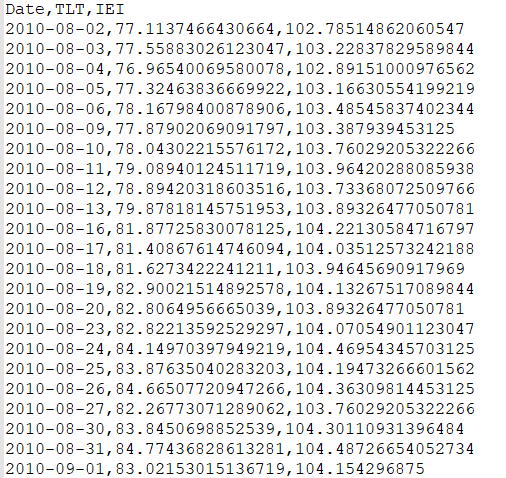
\includegraphics[height=10cm]{images/f000055}
\end{figure}
卡尔曼滤波程序如下所示:
\lstset{language=PYTHON, caption={卡尔曼滤波示例}, label={c000014}}
\begin{lstlisting}
    def hedge_ratio(self):
        etfs = ['TLT', 'IEI']
        start_date = "2010-8-01"
        end_date = "2016-08-01"
        # 获取调整后的收盘价
        dateparse = lambda x: pd.datetime.strptime(x, '%Y-%m-%d')
        prices = pd.read_csv('./work/aqt005_001.txt', encoding='utf-8', parse_dates=['Date'], date_parser=dateparse, index_col='Date')
        # 画散点图
        self.draw_date_coloured_scatterplot(etfs, prices)
        state_means, state_covs = self.calc_slope_intercept_kalman(etfs, prices)
        self.draw_slope_intercept_changes(prices, state_means)
        
    def draw_date_coloured_scatterplot(self, etfs, prices):
        """
        生成散点图,以交易对中两个标的为坐标轴,可以直观观察两个标的间的关系,并且
        采用黄色代表早期数据而红色代表近期数据
        @param etfs 标的字符列表
        @param prices 价格列表,每行为日期、TLT价格、IEI价格
        """
        plen = len(prices)
        colour_map = plt.cm.get_cmap('YlOrRd')
        colours = np.linspace(0.1, 1, plen)
        # 生成散点图
        scatterplot = plt.scatter(
        prices[etfs[0]], prices[etfs[1]],
        s=30, c=colours, cmap=colour_map,
        edgecolor='k', alpha=0.8
        )
        # 添加颜色图表
        colourbar = plt.colorbar(scatterplot)
        colourbar.ax.set_yticklabels(
        [str(p.date()) for p in prices[::plen//9].index]
        )
        plt.xlabel(prices.columns[0])
        plt.ylabel(prices.columns[1])
        plt.show()
        
    def calc_slope_intercept_kalman(self, etfs, prices):
        """
        使用卡尔曼滤波器预测对冲比例
        """
        delta = 1e-5
        mu0 = np.zeros(2)
        sigma0 = np.ones((2, 2))
        Q = delta / (1 - delta) * np.eye(2)
        At = np.eye(2)
        Ct = np.vstack(
            [prices[etfs[0]], np.ones(prices[etfs[0]].shape)]
        ).T[:, np.newaxis]
        R = 1.0
        kf = KalmanFilter(
            n_dim_obs=1,
            n_dim_state=2,
            initial_state_mean=mu0,
            initial_state_covariance=sigma0,
            transition_matrices=At,
            observation_matrices=Ct,
            observation_covariance=R,
            transition_covariance=Q
        )
        
        yt = prices[etfs[1]].values
        #state_means, state_covs = kf.em(observations).filter(observations)
        xt_means, xt_covs = kf.em(yt).filter(yt)
        return xt_means, xt_covs
        
    def draw_slope_intercept_changes(self, prices, state_means):
        """
        绘制斜率和截距
        """
        pd.DataFrame(
            dict(
                slope=state_means[:, 0],
                intercept=state_means[:, 1]
            ), 
            index=prices.index
        ).plot(subplots=True)
        plt.show()
\end{lstlisting}
我们首先从数据文件中读出调整后的收盘价格数据,然后以TFT为横轴,IEI为纵轴,绘制出这两个标的间的对应关系。如下所示:
\begin{figure}[H]
	\caption{散点图}
	\label{f000056}
	\centering
	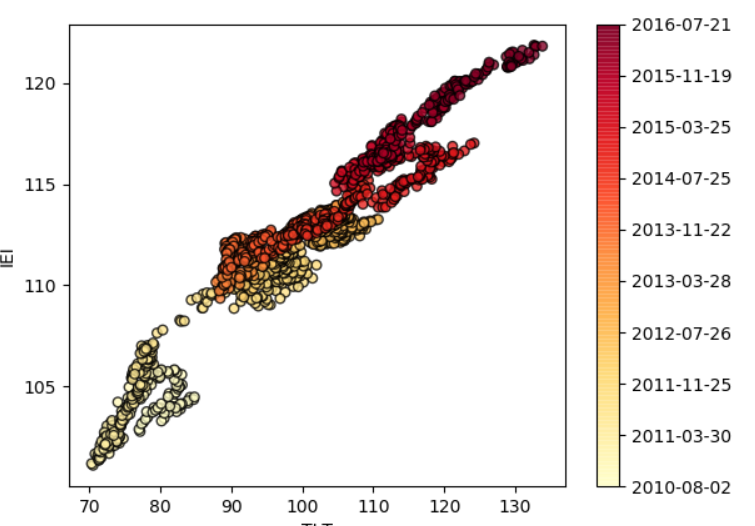
\includegraphics[height=10cm]{images/f000056}
\end{figure}
由图\ref{f000056}可以看出,二者之间有一个相对稳定的线性关系,这是我们应用交易对交易策略的基础。\newline
我们接着利用卡尔曼滤波来预测对冲比例,为了讲述方便,我们把PyKalman库中的公式重新列在这里:
\begin{equation}
\boldsymbol{x}_{t-1}=A_{t}\boldsymbol{x}_{t-1} + \boldsymbol{b}_{t} + \boldsymbol{\epsilon}_{t}^{1}
\label{e000077}
\end{equation}
\begin{equation}
\boldsymbol{y}_{t}=C_{t}\boldsymbol{x}_{t} + \boldsymbol{d}_{t} + \boldsymbol{\epsilon}_{t}^{2}
\label{e000078}
\end{equation}
\begin{equation}
\boldsymbol{\epsilon}_{t}^{1} \in \mathcal{N} \big( 0, Q \big)
\label{e000079}
\end{equation}
\begin{equation}
\boldsymbol{\epsilon}_{t}^{2} \in \mathcal{N} \big( 0, R \big)
\label{e000080}
\end{equation}
我们将TLT的价格,后面加上1之后形成向量,将当前所有时间点的向量组合到一起,形成的矩阵作为观察矩阵,即公式中的$C_{t}$。观察$y_{t}$在这里为1维,因此初始时其协方差矩阵为1。我们按照给定的初始初始化一个卡尔曼滤波器对象,首先调用em()方法对参数进行估计,然后利估计出的参数,运行滤波功能,得到本时刻系统状态即对冲比例。对于每个时间点,其公式为:
\begin{equation}
y_{t}=\begin{bmatrix}
c_{t} & 1
\end{bmatrix}\begin{bmatrix}
x_{t,1} \\
x_{t,2}
\end{bmatrix} \quad => \quad IEI.price=\begin{bmatrix}
TLT.price & 1
\end{bmatrix}\begin{bmatrix}
slope \\
intercept
\end{bmatrix}
\label{e000081}
\end{equation}
注意:在上式中,我们将截距项$\boldsymbol{d}_{t}$作为向量中的一维来表示,因此式中就没有这一项了。\newline
运行上面的程序,就可以得到各个时间点的斜率和截距,我们接着绘制斜率和截距随时变化的曲线,如下所示:
\begin{figure}[H]
	\caption{对冲比例变化曲线}
	\label{f000057}
	\centering
	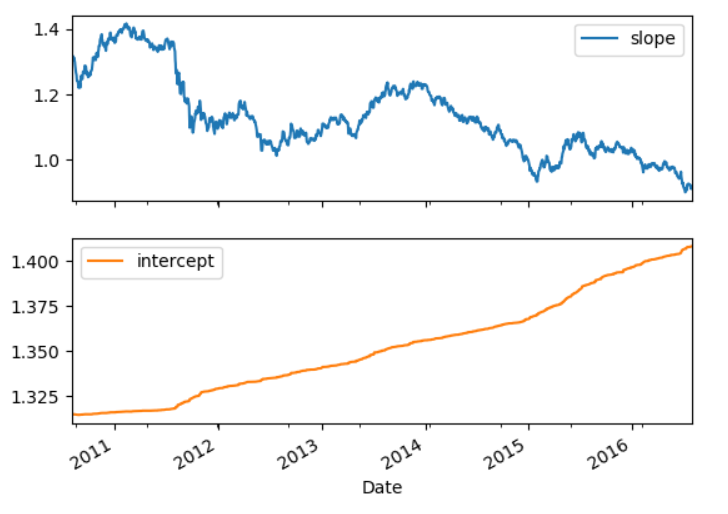
\includegraphics[height=10cm]{images/f000057}
\end{figure}
图\ref{f000057}中,上面蓝色的曲线为对冲比例变化曲线,可以看出,对冲比例并不是一成不变的,因此如果我们按照动态变化的对冲比例来设计交易策略,我们可以得到更高的收益。
